\chapter{Maschinen}

\newpage

\section{DC-Maschine}

\begin{figure}[h!]
\centering
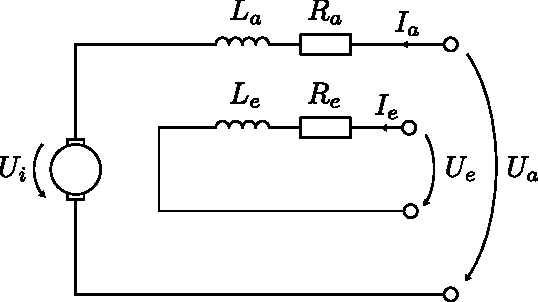
\includegraphics[scale=\schscale]{dc-motor.pdf}
\caption{Ersatzschaltbild einer DC-Maschine}
\label{sch:dc-maschine}
\end{figure}

\subsection{Verhalten und Kennlinie}

Eine DC- oder Gleichstrommaschine hat grundsätzlich drei Betriebszustände:
\begin{itemize}
	\item Ankerstellbereich
	\item Normbereich
	\item Feldschwächungsbereich
\end{itemize}

\begin{figure}[h!]
\centering
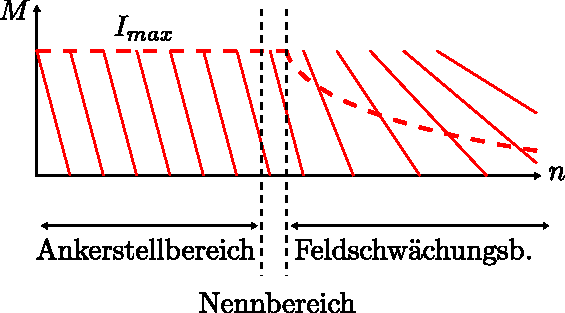
\includegraphics[scale=\schscale]{dc-motor-plot1.pdf}
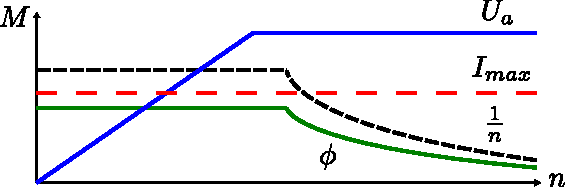
\includegraphics[scale=\schscale]{dc-motor-plot2.pdf}
\caption{Kennlinie einer DC-Maschine}
\label{fig:dc-motor-kennlinie}
\end{figure}

\noindent
Wichtig sind die foldengen Charakteristiken einer DC-Maschine:

\begin{itemize}
	\item Die Drehzahl ist proportional zur Spannung (falls unbelastet).
	\item Nimmt man der DC-Maschine Moment ab (d.h. belasten), so sinkt
		die Drehzahl linear ab bis hin zum maximalen Strom.
	\item	Blockiert man die Rotation (Reibung, Last) so überhitzt
		der Motor.
\end{itemize}

\subsection{Dynamischer Betrieb}
\[ \begin{array}{l}
U_a = U_i + (R_a \cdot I_a) + \left(L_a \cdot \frac{d I_a}{d t}\right) \\\\
U_e = (R_e \cdot I_e) + \left(L_e \cdot \frac{d I_e}{d t}\right) \\\\
U_i = c \cdot \Phi \cdot \omega_m \\\\
M_{el} = c \cdot \Phi \cdot I_a \\\\
M_{el} = M_{Welle} + M_{Reibung} + \left( J \cdot \frac{d \omega_m}{d t} \right) \\\\
\Phi = \frac{L_e}{N_e} \cdot I_e
\end{array} \]

\subsection{Stationärer Betrieb}
\[ \begin{array}{l}
U_a = U_i + (R_a \cdot I_a) \\\\
U_a = (c \cdot \phi \cdot \omega_m) + (R_a \cdot I_a) \\\\
\omega_m 
	= \frac{U_a - (R_a \cdot I_a)}{c \cdot \phi}
	= \frac{U_a}{c \cdot \phi} - \frac{R_a}{c \cdot \phi} \cdot I_a
	= \frac{U_a}{c \cdot \phi} - \frac{R_a}{(c \cdot \phi)^2} \cdot M
\end{array} \]

\newpage

\section{Serieerregte DC-Maschine}\label{sec:dc-motor-serie}

\begin{figure}[h!]
\centering
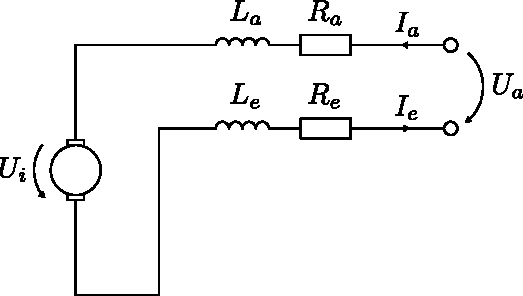
\includegraphics[scale=\schscale]{dc-motor-serie.pdf}
\caption{Ersatzschaltbild der serieerregten DC-Maschine}
\label{sch:dc-maschine-serie}
\end{figure}

\[ I_e = I_a \]
\[ \phi = \frac{L_e}{N_e} \cdot I_e = \frac{L_e}{N_e} \cdot I_a \]
\[ \omega_m = \frac{U_a - (R_a + R_e) \cdot I_a}{c \cdot \frac{L_e}{N_e} \cdot I_a} \]
\[ M_{el} = c \cdot \frac{L_e}{N_e} \cdot I_a^2 \]
\[ U_a = (R_a + R_e) \cdot I_{e,a} + U_i + (L_a + L_e) \cdot \frac{d I}{d t} \]
\[ U_i = c \cdot \frac{L_e}{N_e} \cdot I \cdot \omega_m \]
\[ \omega_m = \frac{U_a - (R_a + R_e) \cdot I}{c \cdot \frac{L_e}{N_e} \cdot I} \]
\[ \omega_m \approx \frac{U_a}{c \cdot \frac{L_e}{N_e} \cdot \sqrt{\frac{N_e \cdot M}{c \cdot L_e}}} 
	= \frac{U_a}{\sqrt{c \cdot \frac{L_e}{N_e}}} \cdot M \]

\newpage

\section{Universalmotor}

Diese elektrische Maschine kann sowohl mit DC als auch mit AC betrieben
werden ohne Veränderungen vorzunehmen, deshalb werden die Doppelnamen 
\textit{Serieerregte Gleichstrommaschine} und 
\textit{Einphasen-Reihenschluss"-motor} benutzt.

Wird die Maschine mit DC betrieben, so gelten die Formeln aus dem Kapitel
\ref{sec:dc-motor-serie}. Wird die Maschine mit AC betrieben, so müssen die
folgenden Formeln benutzt werden.

\[ \underline{U} = (R_a + R_e) \cdot \underline{I} + j \cdot \omega \cdot (L_a + L_e) \cdot \underline{I} + \underline{U_i} \]
\[ \underline{U_i} = c \cdot \phi \cdot \omega_m = c_1 \cdot \underline{I} \cdot \omega_m \]
\[ |\underline{U^2}| = (|U_i| + R \cdot |\underline{I}|)^2 + (\omega \cdot L \cdot |\underline{I}|)^2, \quad U_i = c_1 \cdot |\underline{I}| \cdot \omega_m \]

\begin{figure}[h!]
\centering
\caption{Zeigerdiagramm des Universalmotors bei AC-Betrieb}
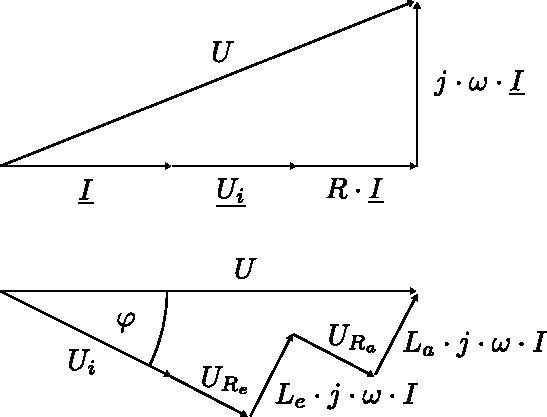
\includegraphics[scale=\schscale]{dc-motor-serie-plot1.pdf}
\label{fig:universalmotor-zeiger}
\end{figure}

\section{Synchronmaschine}
\[ \omega_{mech} = \omega_{D_1} = \frac{\omega_1}{p} \]
\[ p\text{: Polpaarzahl} \]
\[ \omega_1 = f_1 \cdot 2 \pi \qquad \text{elektrischer Kreis} \]
$\qquad$ Index-Bedeutung: $1$: Statorgrössen $D$: Drehfeld
\[ n = \frac{60 \cdot \omega_{mech}}{2 \pi} \]
Beispiel $f_1 = 50 Hz$: 
\[ \begin{array}{@{}c|c}
p & n    \\
\hline
1 & 3000 \\
2 & 1500 \\
3 & 1000 \\
4 & 750  \\
5 & 500  \\
\end{array} \]

\subsection{Ersatzschaltung}
Die folgenden Berechnungen basieren auf folgenden Vereinfachungen: 
\begin{itemize}
  \item stationärer Betrieb, d.h. $\omega_1 = p \cdot \omega_{mech}$
  \item $R = 0$
  \item symmetrisch $\rightarrow$ einphasiges Ersatzschaltbild
\end{itemize}
%%%%%%%%%%%%%%%%%%%%%%%%%%%%%%%%%%%%%%%%
% Hier Bild einfügen
%%%%%%%%%%%%%%%%%%%%%%%%%%%%%%%%%%%%%%%%
\[ x_d = \underbrace{x_a}_{\text{Hauptreaktanz}} + \underbrace{x_{\delta}}
_{\text{Streureaktanz}}\qquad \text{Reaktanzen} \]
$\underline{U_1}$: Phasenspannung \\
$\underline{U_p}$: Polradspannung

\subsection{Inselbetrieb}
%%%%%%%%%%%%%%%%%%%%%%%%%%%%%%%%%%%%%%%%
% Hier Bild einfügen
%%%%%%%%%%%%%%%%%%%%%%%%%%%%%%%%%%%%%%%%
\[ \underline{U_1} + \Delta \underline{U} = \underline{U_p} \]
\[ -\underline{I_1} \cdot \underline{Z} + j x_d \cdot \underline{I_1} 
= \underline{U_p} \]
Leistungen: $P, Q$: Drehstromleistung
\[ P = 3 \cdot Re(\underline{U_1} \cdot (-\underline{I_1})^2) \]
\[ P = 3 \cdot \Re(\underline{U_1} \cdot (-\underline{I_1})^2) \]
\[ Q = 3 \cdot Im(\underline{U_1} \cdot (-\underline{I_1})^2) \]
\[ Q = 3 \cdot \Im(\underline{U_1} \cdot (-\underline{I_1})^2) \]

\subsection{Verbundbetrieb}
%%%%%%%%%%%%%%%%%%%%%%%%%%%%%%%%%%%%%%%%
% Hier Bild einfügen
%%%%%%%%%%%%%%%%%%%%%%%%%%%%%%%%%%%%%%%%
\[ \underline{U_1} = \underbrace{\underline{I_1} \cdot j x_d}_{\Delta U} + U_p \]

\subsection{Polradwinkel $\vartheta$}
\[ \vartheta = \varphi U_1 - \varphi_{U_{p_{U_1}}} \]
\[ \begin{array}{@{}lll}
\vartheta > 0 & \rightarrow & \text{Motorbetrieb} \\
\vartheta < 0 & \rightarrow & \text{Generatorbetrieb} \\
\vartheta = 0 & \rightarrow & \text{Leerlauf} \\
\end{array} \]

\subsection{Drehmoment}
\[ M = \frac{3 \cdot p \cdot U_1 \cdot U_p}{\omega_1 \cdot x_d} 
\cdot \sin{\vartheta} \]

\subsection{Mechanische Leistung}
\[ P_{mech} = \omega_{mech} \cdot M \]

\section{Asynchronmaschine}
Stator: 
\[ \omega_1 = 2 \pi \cdot f_1 \]
\[ \omega_{D_1} = \frac{\omega_1}{p} \qquad p\text{: Polpaarzahl} \]
Synchrone Drehzahl: 
\[ n_{syn} = \frac{60 \cdot \omega_{D_1}}{2 \pi} = \frac{60 \cdot f_1}{p} \]
Rotor: 
\[ \omega_{mech} = \frac{2 \pi \cdot n}{60} \]
\[ \omega_{D_2} = \omega_{D_1} - \omega_{mech} = \frac{\omega_{D_2}}{p} 
\qquad n\text{: Rotordrehzahl} \]
Schlupf: 
\[ S = \frac{n_{syn} - n}{n_{syn}} = \frac{\omega_2}{\omega_1} 
\qquad \text{$\omega_2$: el. Kreisfrequenz der Rotorgrössen $U_2, \varphi_2$} \]
Im Rotor induzierte Spannung: 
\[ \begin{array}{@{}l@{}l@{}l@{}}
U_{n_1} = N_1 \cdot \frac{d \phi_n}{d t} & \Rightarrow 
& U_{n_1} = \omega_1 \cdot N_1 \cdot \phi_n \\
&& U_{n_2} = \omega_2 \cdot N_2 \cdot \phi_n \\
\end{array} \]
\[ ü = \frac{N_1}{N_2} \]
\[ U_{n_2} = N_2 \cdot \omega_2 \cdot \frac{U_{n_1}}{N_1 \cdot \omega_1} 
= \frac{S \cdot U_{n_1}}{ü} \]
\[ \begin{array}{@{}lll}
S < 0     & \rightarrow & \text{Übersynchron} \\
S = 0     & \rightarrow & \text{Synchron} \\
0 < S < 1 & \rightarrow & \text{Untersynchron} \\
S = 1     & \rightarrow & \text{Stillstand} \\
S > 1     & \rightarrow & \text{Gegenlauf} \\
\end{array} \]

\subsection{Leistungen}
(ideales Modell, kein magn. Strom, streuungsfrei)\\
Stator: 
\[ P_1 = 3 \cdot U_{n_1} \cdot I_1 \]
Luftspalt: 
\[ P_\delta = P_1 - \underbrace{3 \cdot R_1 \cdot {I_1}^2 - P_{Fe}}_
{\text{Falls Statorverlust}} \]
Rotor: 
\[ P_2 = 3 \cdot U_{n_2} \cdot I_2 
= 3 \cdot S \cdot U_{n_1} \cdot I_1 = S \cdot P_\delta \]
\[ \begin{array}{ccccc}
P_1 & \Rightarrow &  P_\delta & \Rightarrow & P_{mech} \\
\Downarrow & & \Downarrow & & \\
3 \cdot R_1 \cdot {I_1}^2 + P_{Fe} & & P_2 & \\
\end{array} \]

\subsection{Betriebsarten}
Motor: 
\[ \begin{array}{llllll}
0 < S < 1 
  & 0 < n < n_{syn} 
  & P_\delta > 0 
  \\ 0 < P_{mech} < P_1 
  & 0 < P_2 < P_\delta 
  & \eta = \frac{P_{mech}}{P_1} < 1 - S
\end{array} \]
Generator: 
\[ \begin{array}{llllll}
S < 0 
  & n > n_{syn} 
  & P_\delta < 0 
  \\ P_{mech} < 0 
  & P_2 > 0
  & \eta = \frac{P_1}{P_{mech}} < \frac{1}{1 - S}
\end{array} \]
Gegenlauf: 
\[ \begin{array}{llllll}
S > 1 
  & n < 0
  & P_\delta > 0 
  & P_{mech} > 0
  & P_2 > 0
\end{array} \]
